%\documentclass[a4paper, 10pt]{article}
\documentclass[paper=a4, fontsize=11pt]{article}
\usepackage[brazil]{babel}
\usepackage[utf8]{inputenc}
\usepackage{listings}
\usepackage{color}
\usepackage{amsthm}
\usepackage{graphicx}
\usepackage{schemabloc}
\usetikzlibrary{circuits}
\usepackage{tabularx,ragged2e,booktabs,caption}

\setlength{\parindent}{0pt}
\setlength{\parskip}{18pt}

\title{\textsc{Detecção de componente continua em transformadores de potência}}
\author{Felipe Bandeira, 1020942-X\\Renan Teixeira, 1010775-0}
%\date{}

\begin{document}


\maketitle

%\begin{abstract}
\textit{A presença de cargas não lineares, sejam, inversores de frequência, grandes computadores. Introduzem na rede uma distorção da senoide produzida pela geradores de energia. Essa componente DC injetada na alimentação de transformadores de potência, satura o núcleo do transformador, aumenta a temperatura interna do mesmo. Danificando em muitos casos a isolação. Esse resumo do artigo tem como principal objetivo: detectar a saturação magnetica por um metodo não diretor de medição de corrente continua. E outras palavras a somatória das componentes DC dos equipamento conectados no transformador. A sensor magnético desenvolido pelos autores do trabalho, verifica em um loop fechado e com faixa de rejeição os campos magnéticos, com uma boa linearidade. E no final são confrontados os resultados das simulações e experimental confirmando uma otima aproximação em ambos.}
%\end{abstract}

\newpage

\tableofcontents

\newpage

\listoffigures


%%%%%%%%%%%%%%%%%%%%%%%%%%%%%%%%%%%%%%%%%%%%%%%%%%%%%%%%%%%%%%%%%%%%%%%%%%%%%%%%
% fundamentação teórica
\newpage
\section{Introdução}

O aumento do uso de conversores de potência na industria, é razão, em boa parte das 
situações os problemas referidos na qualidade de energia. Um dos maiores motivos 
para as distorções são as cargas não lineares produzidas pelos conversores. Por essa
razão é e são utilizadas diversos filtros ativos ou passivos na tentativa de melhorar
a qualidade da energia. O problema da componente continua na energia elétrica e 
valores tolerados, varia de pais ou região, os limites são regulados pelas normas 
locais. Entretanto o seguimento das normas não é garantia de correção para esse problema.
É relativamente impossível abrir mão dos conversores de potência nos dias atuais, 
então deve-se trabalhar em cima das harmônicas produzidas e uma forma de correção.
No artigo aqui apresentado o alvo para a analise dos problemas causados pela componente
DC são os transformadores de potência. O principal problema a injeção de corrente 
continua em transformadores é a saturação assimétrica do núcleo magnético durante 
meio ciclo. Quando essa condição é presente o consumo de energia reativa cresce, 
implicando em perda de potência e consequentemente no aumento da temperatura do
transformador. Os autores deste artigo propõem um método indireto e on-line 
de detecção da componente continua injetada no transformador. A literatura
apresenta diversas  alternativas on-line e offline no diagnostico na detecção 
de falhas e monitoramento. Existem métodos que verificam instantaneamente 
curtos em vários estágios da transmissão, mensuramento apenas o fluxo de 
corrente do transformador. Outra técnica é baseada na analise da função de transferência
do circuito, quando injetando um sinal conhecido, verifica-se tensões internas
nos taps do transformado tensões externa, fazendo isso a diferenciação entre
erros internos do transformado e erros externos. Em particular a medição de componente
continua injetada em sistemas de potência, não são muito exploradas na literatura.

A principal ideia e proposta do artigo é quando a componente continua flui pelo
transformador existem quedas de tensão na resistências parasitas dos enrolamentos.
Essa queda de tensão continua, guarda informações valiosas sobre a saturação
no núcleo do transformador. Essa queda de tensão entretanto é muito pequena (para um
transformador de potência a resistência dos enrolamentos é da ordem de miliohns), 
sensores tradicionais não são capazes de detectar a componente continua, já que 
são exclusivamente voltados para a medição AC. Entretanto a utilização dos sensores
de efeito Hall apresenta pequenos problemas, existem uma grande dificuldade de 
separar a componente DC muito pequena das componentes AC grandes. Os autores do 
artigo criaram um sensor magnético não linear com uma grande sensibilidade para
componente DC. Mensurando assim, as pequenas componentes DC encontrada na resistências
parasitas dos enrolamentos do transformador. Os autores apresentam duas diferentes
implementações para  a medição. Uma é em malha aberta e outra em malha fechada. 
A primeira opera na medição do fluxo de DC dentro do sensor do núcleo(em malha
fechada é visto o fluxo de harmônicas). A simulação e os resultados experimentais
confirmam a eficiência do método. Em particular os ótimos resultados adquiridos no 
métodos da malha fechada.

\section{Principio de operação}

O elemento chave proposto é um sensor com alta precisão para mediação de corrente
continua com uma razão de rejeição em modo comum alta. Lembrando que o sensor 
é capaz de extrair uma componente continua na ordem de milivolts de um sinal
com tensão de pico a pico na ordem de 600 $V_{rms}$. O sensor feito pelos autores
é composto por um núcleo toroidal, com dois enrolamentos e um reator para a compensação.
A componente magnética é quantificada, imitando a baixa potência do transformador
toroidal com a tensão primária. O secundário é então utilizado para garantir o 
loop fechado. O modelo para o componente magnético do sensor, chamado pelos autores
de reator simples, é apresentado na Figura~\ref{fig:figura1}.

\begin{figure}[!ht]
	\centering
	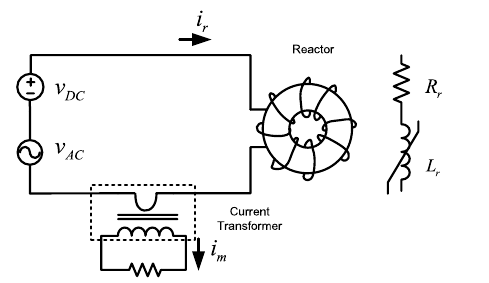
\includegraphics[scale=.8]{fig1.png}
    \caption{Esquemático do reator, conectado a fonte AC com a componente DC}
    \label{fig:figura1}
\end{figure}

A figura~\ref{fig:figura1} mostra um resistência em séria uma indutância não linear
o enrolamento secundário não é considerado ainda, o reator é então conectado a
uma fonte de corrente AC com uma componente DC. A corrente $i_R$ do reator, é
detectada por um transformador de corrente. O transformador de corrente
é implementado para a correção do offset na medição. Para uma baixa qualidade na 
medição um simples resistor shunt pode ser utilizado.
A operação do sensor é atuante na saturação assimétrica apresentando assim a componente
DC no funcionamento em regime permanente do transformador. A figura ~\ref{fig:figura2} 
mostra as formas de onda para o fluxo magnético no reator, corrente de magnetização
quando uma componente continua esta presente na rede. Nota-se que o fluxo magnético é
mais intenso no fim do semiciclo da senoide.

\begin{figure}[!ht]
	\centering
	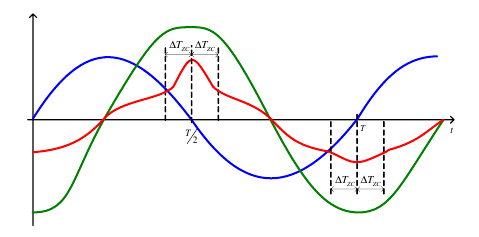
\includegraphics[scale=.8]{fig2.png}
    \caption{Tensão do reator(azul), fluxo magnético(verde) e corrente de magnetização(vermelho), na presença da componente DC.}
    \label{fig:figura2}
\end{figure}

O resultado apresenta que, quando a corrente do reator presente for alta é correspondente
ao semi ciclo positivo ou negativo dependente da componente DC. A saturação assimétrica
do núcleo é informada pela componente DC em amplitude. Para detectar a distorção
assimétrica em todo os ciclos da senoide é feita uma integração para a saturação positiva
e negativa em um ponto bem próximo a transição do zero.

No caso da tensão DC seja positiva equivale a semi ciclo positivo do fluxo de saturação e
a distorção assimétrica, equivalente as harmônicas pares. No caso do modulo da integral
para o semi ciclo positivo seja maior que o modulo da integral para o semi ciclo negativo
a valor e sinal para a a componente DC. A corrente que flui para transformador de
corrente e totalmente imune as variações de offset. No caso o transformador de corrente
retira toda a componente DC, logo, não poderá ser vista nenhum sinal DC. Partindo desta
premissa o circuito digital é capaz de aumentar rejeição em modo comum.
Em outras palavras a detecção da componente continua pode ser vista na figura ~\ref{fig:figura3}

\begin{figure}[!ht]
	\centering
	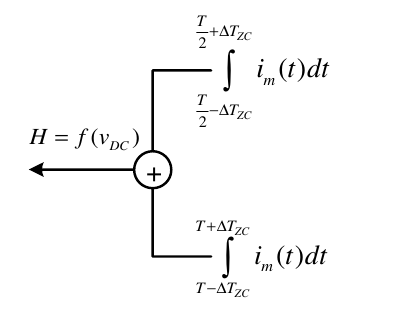
\includegraphics[scale=.8]{fig3.png}
    \caption{Detector da componente DC}
    \label{fig:figura3}
\end{figure}

A função $H$ guarda as informações para a componente DC. Importante notar que os 
altos niveis de saturação não devem ser capazes de modificar a linearidade do 
circuito, por isso o sensor desenvolvido é altamente linear para uma vasta gama 
de valores. O método para o loop fechado apresenta uma resposta mais dinâmica e 
bem mais. A figura ~\ref{fig:figura4} exemplifica todo o processo de aquisição 
da componente DC

\begin{figure}[!ht]
	\centering
	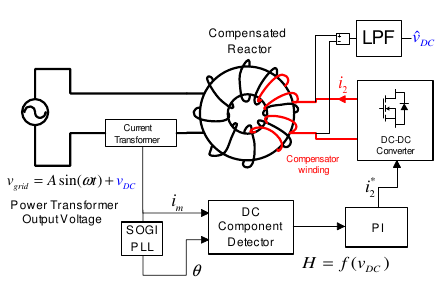
\includegraphics[scale=.8]{fig4.png}
    \caption{Estrutura de controle}
    \label{fig:figura4}
\end{figure}

\section{Resultado das simulações}

O sensor proposto foi simulado usando o ambiente Matlab/Simulink. O esquemático mostrado
na figura ~\ref{fig:figura4} foi implementado. Todos os sinais foram simulados em
um tempo de 100 us, e implementado em um DSP de baixo custo. A simulação foi feita 
em 2 passos. Primeiro, foi solucionado para dependente da função $H=f(V_{DC})$ para 
o conversor DC sem o uso a bobina de compensação, ou seja, em malha aberta. Enquanto
a segunda simulação foi feita usando a bobina de compensação(em malha fechada).
O compensador foi implementado usando um controlador PI com o tempo de amostragem igual
a 20ms. $SI_P$ e $SI_N$ são atualizados em cada semiciclo da tensão. Para as características
da magnetização do reator(referente a bobina do primário) mostrada na figura ~\ref{fig:figura6}.

\begin{figure}[!ht]
	\centering
	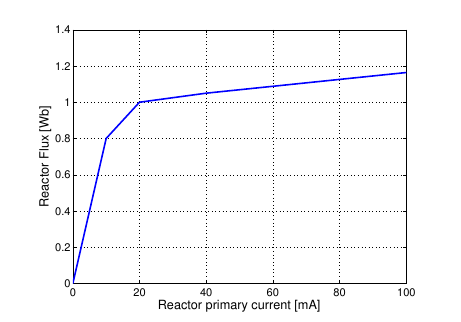
\includegraphics[scale=.8]{fig6.png}
    \caption{Características de magnetização, referente a bobina do primário}
    \label{fig:figura6}
\end{figure}

A resistência da bobina foi considerada de 30 ohms. Esse valor é alto, valor escolhido
de tal forma que o sistema seja capaz de responder a uma grande variação do campo magnético
A relação de espiras entre o enrolamento primário e de compensação foi 1:3000.

Os resultados da simulação são apresentados na figura ~\ref{fig:figura7} e ~\ref{fig:figura8}.

\begin{figure}[!ht]
	\centering
	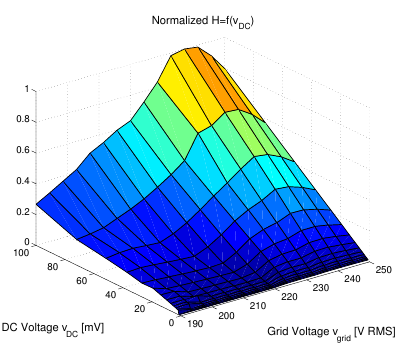
\includegraphics[scale=.8]{fig7.png}
    \caption{Componente DC normalizada, em malha aberta}
    \label{fig:figura7}
\end{figure}


\begin{figure}[!ht]
	\centering
	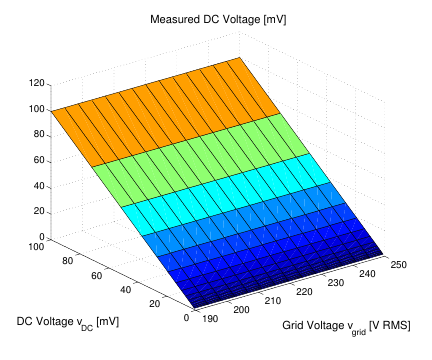
\includegraphics[scale=.8]{fig8.png}
    \caption{Component DC normalizada, em malha fechada}
    \label{fig:figura8}
\end{figure}

No caso do sistema em malha aberta o valor absoluto de H não é significante devido
as fontes não lineares, então foi normalizado para o valor máximo. Enquanto que
o circuito em malha fechada(veja figura ~\ref{fig:figura4}) a tensão é $V_{DC}$.
É evidente que sem a compensação, há uma forte dependência da tensão da 
amplitude da rede na polarização DC. A sensibilidade máxima é atingida
em torno da tensão nominal de 230 $V_{RMS}$. Para valores inferiores 
do reator é menos saturado. Enquanto que a partir dos valores mais elevados
o efeito da polarização DC são amortecidas através da resistência parasitas.

\section{Aplicação do sensor em transformadores de potência}

A seções anteriores mostraram a capacidade do sensor e sua alta sensibilidade
para pequenos valores da componente DC. Para a sua aplicação em transformadores
comumente encontrados em sistemas de distribuição se faz necessário a criação
de implementação de 3 sensores para um sistema de trifásico, 4 fios(neutro incluso).

\section{Resultados experimentais}

E por fim os autores implementaram o sistema na pratica, com o intuito de concretizar
a ideia aqui exposta. O prototipo tem como base a figura ~\ref{fig:figura4}. Para
implementar o conversor não linear foi utilizado um controle de motor de 24V 300W.
A placa do DSP foi DSP MC56F8037 da Freescale. O prototipo para o reator foi
construido e é mostrada na figura ~\ref{fig:figura11}. 

\begin{figure}[!ht]
	\centering
	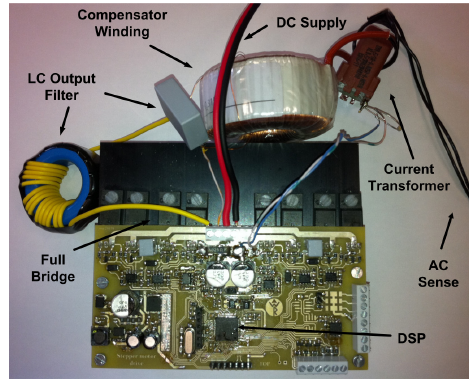
\includegraphics[scale=.8]{fig11.png}
    \caption{Prototipo para o compensador}
    \label{fig:figura11}
\end{figure}

O compensador foi conectado a um transformador de 3 kVA e para aumentar o níveis 
de teste foi inserido um autotransformador. A fonte de componente continua foi
projetada para injetar 1kW de potência ativa. O esquemático para os teste
é mostrado na figura ~\ref{fig:figura12}.

\begin{figure}[!ht]
	\centering
	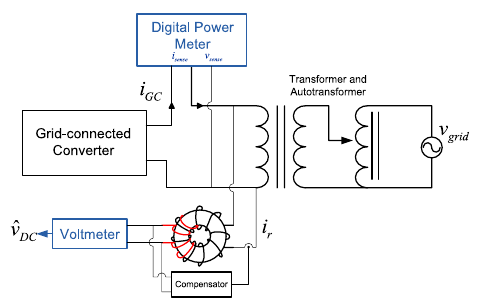
\includegraphics[scale=.8]{fig12.png}
    \caption{Esquemático do teste}
    \label{fig:figura12}
\end{figure}


\begin{figure}[!ht]
	\centering
	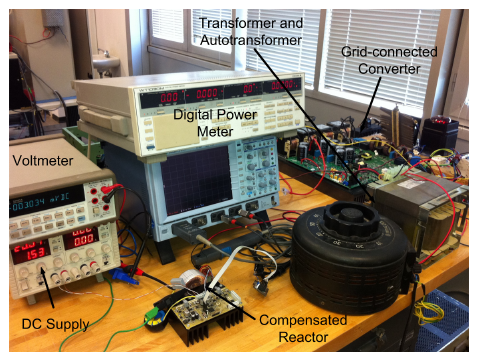
\includegraphics[scale=.8]{fig13.png}
    \caption{Prototipo final}
    \label{fig:figura13}
\end{figure}

Outra forma de avaliar a eficiência do sistema é mensurando a tensão na bobina versus
a componente DC injetada. Durante os experimentos a temperatura do transformador foi
mantida em valores constantes. Um forma de diminuir a variações da resistência 
parasita. Os resultados das medições é mostrado na figura ~\ref{fig:figura14} ficando
evidente a compensação do sistema garante a alta linearidade do sistema.
A figura ~\ref{fig:figura16} mostra as formas de ondas obtidas para o
prototipo em pleno funcionamento.
\begin{figure}[!ht]
	\centering
	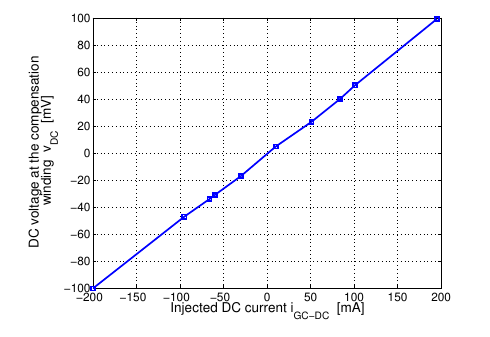
\includegraphics[scale=.8]{fig14.png}
    \caption{Forma de onda para pleno funcionamento}
    \label{fig:figura14}
\end{figure}


\begin{figure}[!ht]
	\centering
	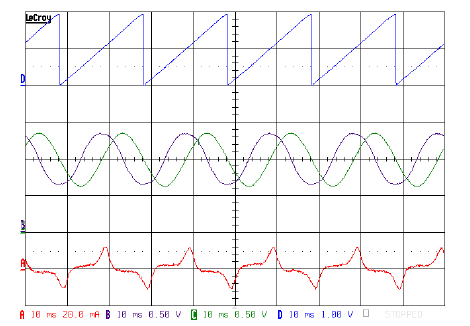
\includegraphics[scale=.8]{fig16.png}
    \caption{Forma de onda para pleno funcionamento}
    \label{fig:figura16}
\end{figure}

\section{Conclusão}

Esse paper tem como principal objetivo mostrar um novo sensor para diagnosticar a 
extensão da componentes de saturação assimétricas em transformadores de potência
devido as componente DC. A principal causa de componentes continuas é o uso
de conversores eletrônicos(fontes de alimentação chaveadas, inversores de frequência,
conversores conectados a rede para a energia renováveis) que causam e ampliam
a componentes harmónicas da senoide da rede. A corrente continua que flui no 
transformador de potência provoca uma queda de tensão na pequena resistência do
enrolamento do transformador. O sensor proposto é capaz de medir e mensurar essa
componente de tensão continua com uma alta sensibilidade e linearidade e livre de
problemas de ruídos e baixo valores desta componente. Os resultados da simulação
mostra uma otima resposta com os valores simulados. E principalmente para o circuito
em malha fechada na presença de variações grande da amplitude da rede.

\end{document}
 
